\section{Hardware Generation}
\label{hardware}

In this section, we describe how the tiled intermediate representation is
translated into an efficient FPGA design. FPGAs are composed of various logic,
register, and memory resources. These resources are typically configured for
a specific hardware design using a hardware description language (HDL)
that is translated into an FPGA configuration file.

To separate concerns of this chapter from the subsequent chapter on Spatial,
and to define a ground set of templates required for Spatial's design,
we describe our approach to FPGA hardware generation here as generation rules
from PPL into a simple set of hardware templates. We describe how
these templates can be further refined
into a full hardware-specific intermediate representation in Chapter~\ref{spatial}.

\begin{table*}[t]
\footnotesize\centering
\begin{tabular}{ |m{1.5cm}|l|m{6cm}|m{3.8cm}| }

\noalign{\hrule height 1.5pt}
\multicolumn{1}{|l}{} &
\multicolumn{1}{c}{\bf Template} &
\multicolumn{1}{c}{\bf Description} &
\multicolumn{1}{c|}{\bf IR Construct} \\
\noalign{\hrule height 1.0pt}

\multirow{3}{1.5cm}[0pt]{\centering \bf Memories}
& Buffer & On-chip scratchpad memory & Statically sized array \\ \cline{2-4}
& Double buffer & Buffer coupling two stages in a metapipeline & Same as metapipeline controller \\ \cline{2-4}
& Cache & Tagged memory to exploit locality in random memory access patterns & Non-affine accesses \\
\noalign{\hrule height 1.0pt}

\multirow{4}{1.5cm}[0pt]{\centering \bf Pipelined Execution Units}
& Vector & SIMD parallelism & Map over scalars \\ \cline{2-4}
& Reduction tree & Parallel reduction of associative operations & MultiFold over scalars \\ \cline{2-4}
& Parallel FIFO & Used to buffer ordered outputs of dynamic size & FlatMap over scalars \\ \cline{2-4}
& CAM & Fully associative key-value store & GroupByFold over scalars \\
\noalign{\hrule height 1.0pt}
%\multicolumn{1}{|l|}{Priority Queue}          & \multicolumn{1}{p{7cm}|}{Pipelined priority insert into a list} & \multicolumn{1}{l|}{Sort} \\ \midrule

%\multicolumn{4}{|c|}{Controllers} \\ \midrule
\multirow{4}{1.5cm}[-10pt]{\centering \bf Controllers}
& Sequential & Controller which coordinates sequential execution & Sequential IR node \\ \cline{2-4}
& Parallel & Task parallel controller. Simultaneously starts all member modules when enabled, signals done when all members finish & Independent IR nodes \\ \cline{2-4}
& Metapipeline & Controller which coordinates execution of nested parallel patterns in a pipelined fashion & Outer parallel pattern with multiple inner patterns \\ \cline{2-4}
& Tile memory & Memory command generator to fetch tiles of data from off-chip memory & Transformer-inserted array copy \\
\noalign{\hrule height 1.5pt}

\end{tabular}
\caption{Simplified hardware templates used in hardware code generation.}
\label{t-hwtemplates}
\end{table*}


Table~\ref{t-hwtemplates} lists the templates and their corresponding PPL IR
constructs in three classes: memories, pipelined execution units,
and state machine controllers. \emph{Buffer}, \emph{Double buffer},
and \emph{Cache} are different on-chip memory templates intended to capture both
regular and data-dependent access patterns. In particular, the \emph{double buffer} template
is used to decouple execution stages and support dynamic rate mismatch between producer and consumer stages. Templates labeled as
\emph{Pipelined Execution Units} are used to support different kinds of innermost parallel patterns, as described in Table~\ref{t-hwtemplates}.
The \emph{Controller} templates implement a specific form of control flow using asynchronous handshaking signals. The \emph{Sequential},
\emph{Parallel}, and \emph{Metapipeline} controllers all orchestrate execution of a list of templates; \emph{Sequential} enforces
linear execution order, \emph{Parallel} enforces parallel execution with a barrier at the end, and \emph{MetaPipeline} enforces
pipelined execution. \emph{Tile Memory} controllers correspond to off-chip memory channels that load tiles of data into
one of the on-chip memory templates.
%We summarize the parallel pattern IR construct whose behavior each template captures in Table~\ref{t-hwtemplates}.
Each template can be composed with other templates.
For example, a \emph{Metapipeline controller} could be composed of multiple \emph{Parallel controller}s, each of which could
contain pipelined \emph{Vector} or \emph{Tree reduction} units.
%Next we discuss each of the templates in more detail.
We next describe the key features in the IR which we use to infer each of these template classes.



%\subsection{Memory Allocation}
\subsection{Memory Allocation}
Generating efficient FPGA hardware requires effective usage of on-chip memories (buffers).
Prior to generating MaxJ, we run an analysis pass to allocate buffers for arrays based on data access patterns and size.
%Since the maximum size of data inputs can not usually be inferred statically, we support the use of programmer hints about tile sizes to aid this analysis.
%Information from these annotations is propagated through the IR during this analysis.
All arrays with statically known sizes, such as array \emph{copies} generated in the tiling transformation described in
Section~\ref{transformations}, are assigned to buffers. Dynamically sized arrays are kept in main memory and we generate
caches for any non-affine accesses to these arrays.
We also track each memory's readers and writers and use this information
to instantiate a template with the appropriate word width and number of ports.

% Special memories are used for buffers which have unique access patterns. Streaming or ``one-touch'' data is
% either streamed directly to and from off-chip memory or realized using FIFOs on-chip depending on their usage.
% The tiling transformations described in Section
% represent data tile copies with explicit nodes in the IR. This greatly simplifies memory allocation analysis.
% to first determine where data
% is stored and how it is accessed.
% The goal of this analysis is to assign buffers
% to either on-chip or off-chip memories and select a memory template based on the properties
% of the buffer.
%In general, we use the following heuristics to allocate memories:
%\begin{itemize}
%  \item Buffers which have statically unknown dimensions (typically inputs and outputs)
%    are allocated off-chip. However, we allow programmers to provide hints to the compiler using
%    annotations which can enable more aggressive compiler optimizations. For example, the programmer
%    can hint that a certain buffer is ``cacheable'' -- meaning that the size of the buffer is typically
%    small enough (a few Kilobytes) to completely fit on-chip. Our analysis makes use of this information
%    and performs more aggressive on-chip memory allocation.
%  \item Buffers corresponding to tiles are allocated on-chip.
%  \item
%  \item Intermediate buffers in a \emph{metapipeline} (described in the next section) are realized
%    using \emph{Double Buffers}.
%\end{itemize}

%While the memory allocation analysis performs an initial assignment of templates to buffers, certain special
%buffers need to be \emph{promoted} to use the double buffer template. This is determined during
%metapipeline analysis, described in the next section.


%\subsection{Pipeline Execution Units}
\subsection{Pipeline Execution Units}
We generate parallelized and pipelined hardware when parallel patterns compute with scalar values,
as occurs for the innermost patterns.
We implemented templates for each
pipelined execution unit in Table~\ref{t-hwtemplates} using MaxJ language
constructs, and instantiate each template with the proper parameters (e.g., data type,
vector length) associated with the parallel pattern.  The MaxJ compiler
applies low-level hardware optimizations such as vectorization, code
scheduling, and fine-grained pipelining, and generates efficient hardware.  For
example, we instantiate a reduction tree for a MultiFold over an
array of scalar values, which is automatically pipelined by the MaxJ compiler.



%\subsection{Metapipelining}
\subsection{Metapipelining}
To generate high performance hardware from parallel patterns, it is insufficient to exploit only a single level of parallelism.
However, exploiting nested parallelism requires mechanisms to orchestrate
the flow of data through multiple pipeline stages while also exploiting parallelism at each stage of execution,
creating a hierarchy of pipelines, or \emph{metapipeline}.
This is in contrast to traditional HLS tools which require inner patterns to have a static size and be completely unrolled in order to generate a flat pipeline containing both the inner and outer patterns.

% The main motivation behind metapipelining is to exploit parallelism at multiple levels of nesting. If
% a parallel pattern does not have other patterns in its body, then the pattern is implemented as a regular multi-stage
% dataflow pipeline. We leverage the pipelining constructs in the MaxJ programming language and the underlying
% MaxCompiler toolchain in order to implement these simpler pipelines.

%Pattern-specific rules to identify metapipeline stages are described in table \ref{table:metapipelineRules}.

%\todo{Introduce... Implementing a parallel pattern as a metapipeline involves multiple steps, as described below:}

\begin{figure*}
\centering
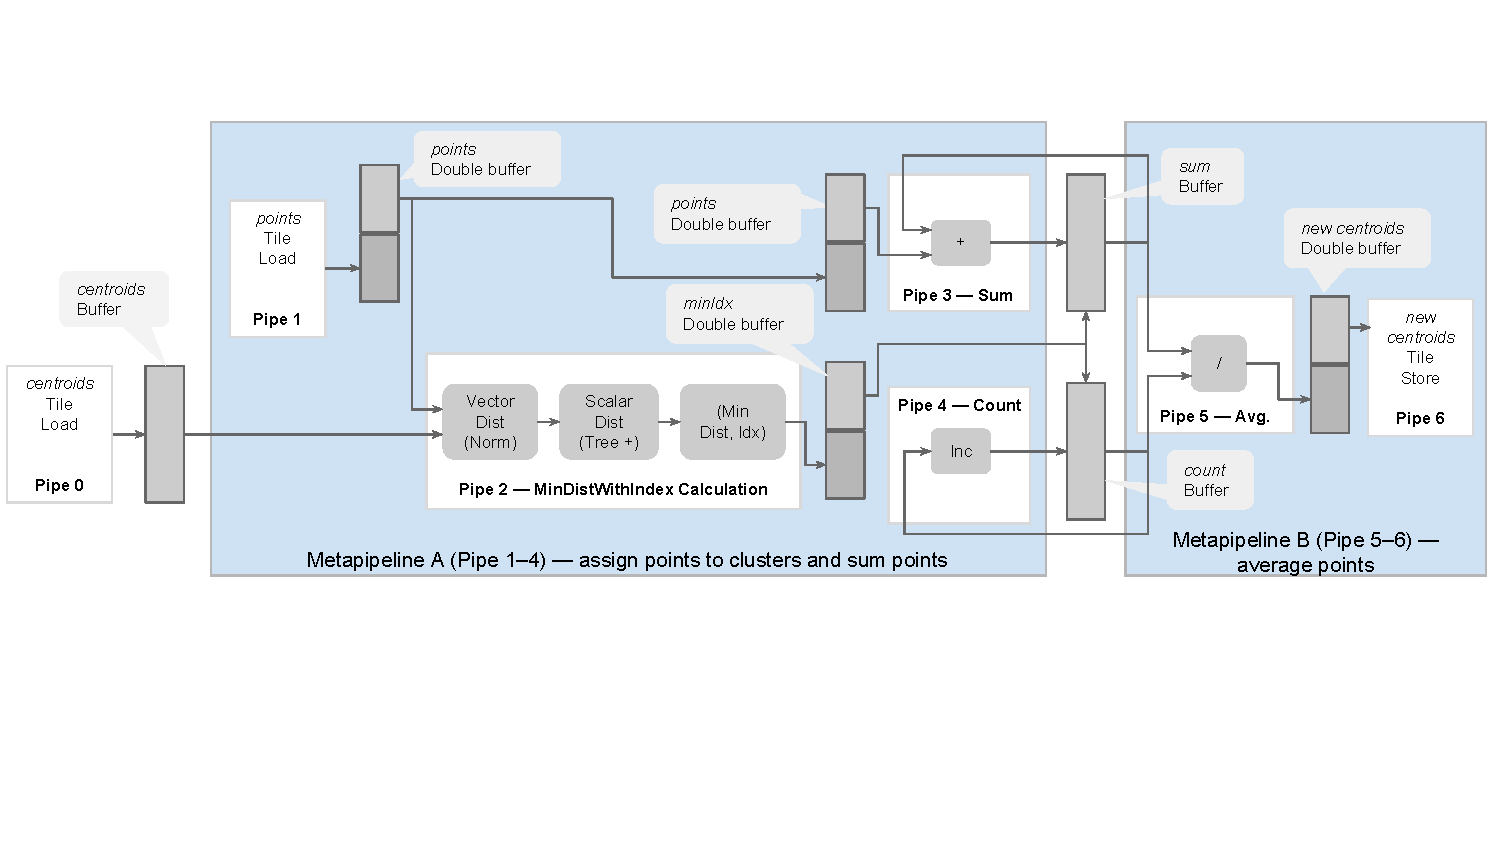
\includegraphics[width=6in]{3-delite/figs/kmeans-blockdiagram.pdf}
\caption{Block diagram of hardware generated for the $k$-means application.}
\label{fig:metapipelining}
\end{figure*}

We create metapipeline schedules by first performing a topological sort on the IR of the body of the current parallel pattern.
The result is a list of stages, where each stage contains a list of patterns which can be run concurrently.
Exploiting the pattern's semantic information, we then
optimize the metapipeline schedule by removing unnecessary memory transfers and redundant computations.
For instance, if the output memory region of the pattern has been assigned to a buffer,
we do not generate unnecessary writes to main memory.

As another example, our functional representation of tiled parallel patterns can sometimes create redundant accumulation functions,
e.g., in cases where a MultiFold is tiled into a nested MultiFold. During scheduling we identify
this redundancy and emit a single copy of the accumulator, removing the unnecessary intermediate buffer.
Finally, in cases where the accumulator of a MultiFold cannot completely fit on-chip, we add a special
forwarding path between the stages containing the accumulator. This optimization avoids redundant writes to memory and
reuses the current tile.
Once we have a final schedule for the metapipeline, we promote every output buffer in each stage
to a double buffer to avoid write after read (WAR) hazards between metapipeline stages.


\subsection{Example}
Figure~\ref{fig:metapipelining} shows a block diagram of the hardware generated for the $k$-means application.
For simplicity, this diagram shows the case where the \emph{centroids} array completely fits on-chip, meaning
we do not tile either the number of clusters \emph{k} or the number of features \emph{d}.
The generated hardware contains three sequential steps.

The first step (Pipe~0) preloads the entire \emph{centroids} array into a buffer.
The second step (Metapipeline A) is a metapipeline which consists of three stages with double buffers to manage communication between the stages.
These three stages directly correspond to the three main sections of the MultiFold (Figure~\ref{fig:kmeans-fused}, line~5) used to sum and count the input points as grouped by their
closest centroid. The first stage (Pipe~1) loads a tile of the \emph{points} array onto the FPGA. Note that this stage is double buffered to
enable hardware prefetching. The second stage (Pipe~2) computes the index of the closest centroid using vector compute blocks and a scalar reduction
tree. The third stage (Pipe~3 and Pipe~4) increments the count for this minimum index and adds the current point to the corresponding location in the
buffer allocated for the \emph{new centroids}.

The third step (Metapipeline B) corresponds with the second outermost parallel pattern in the $k$-means application.
This step streams through the point sums and the centroid counts, dividing each sum by its corresponding count. The resulting new centroids
are then written back to main memory using a tile store unit for further use on the CPU.

Our automatically generated hardware design for the core computation of $k$-means is very similar to the manually optimized design described by Hussain et al.~\cite{hwkmeans}.
While the manual implementation assumes a fixed number of clusters and a small input dataset which can be preloaded onto the FPGA, we use tiling to automatically generate
buffers and tile load units to handle arbitrarily sized data. Like the manual implementation, we automatically parallelize across centroids
and vectorize the point distance calculations. As we see from the $k$-means example, our approach enables us to automatically generate high quality hardware implementations which are comparable to manual designs.
